\chapter{Sistema}

Entre de dispositivos que realizan la clasificación de paquetes se encuentran soluciones implementadas de manera completa en hardware, FPGA, ASIC u otra plataforma, como por ejemplo NetFPGA\cite{netfpga}, o implementadas, procesador de propósito general mediante, completamente en software, que es el caso de Click\cite{click}. La intención de este proyecto integrador, como puede verse de manera gráfica en la figura~\ref{fig:hwsw}, es complementar las ventajas de ambos mundos maximizándolas y reduciendo así las desventajas de utilizar el hardware o el software por separado. 


 \begin{figure}[h]
  \centering
	 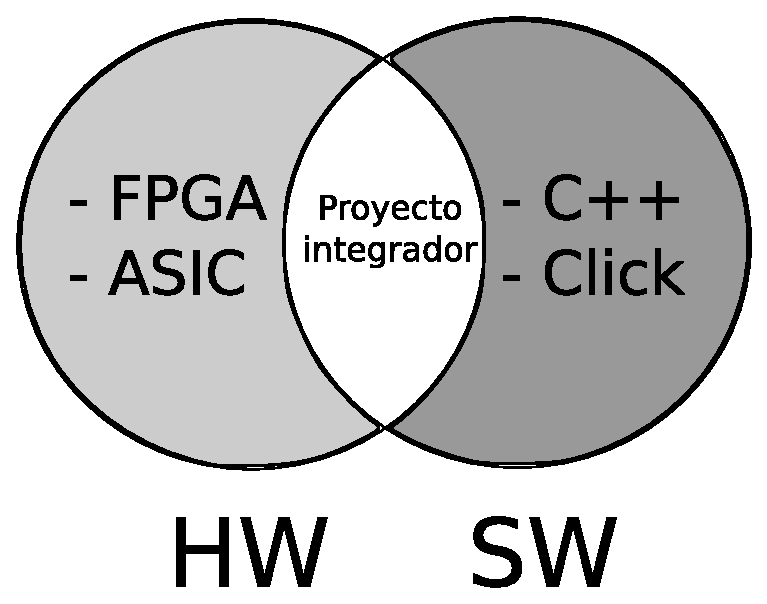
\includegraphics[width=0.6\textwidth]{2-sistema/graf/interseccion.eps}
  \caption{Arquitectura mixta}
  \label{fig:hwsw}
\end{figure}


\section{Solución propuesta}

Para el problema planteado en el capítulo anterior se propone, de manera funcional, la siguiente solución: 

    \begin{enumerate}
  	\item Un flujo de paquetes llega a la interfaz de red del dispositivo y es necesario clasificarlo en distintos flujos para que sea redireccionado.
	\item Se almacenan los paquetes en un buffer según el orden de llegada.
	\item Se extrae el primer paquete y se toma la información que pertenece a la cabecera; La información completa del paquete queda en espera.
	\item Se envía la cabecera al microprocesador.
	\item El microprocesador aplica un algoritmo de clasificación a cierta información de la cabecera y reenvía los resultados al hardware. 
	\item Se envía el paquete a la interfaz de salida, anexándole a cada palabra un tag adjunto con el resultado de la clasificación.
    \end{enumerate}

\section{Esquema propuesto}
Para implementar la solución se propone el hardware descripto en el diagrama de la figura~\ref{fig:solucion}
 \begin{figure}[h]
  \centering
	 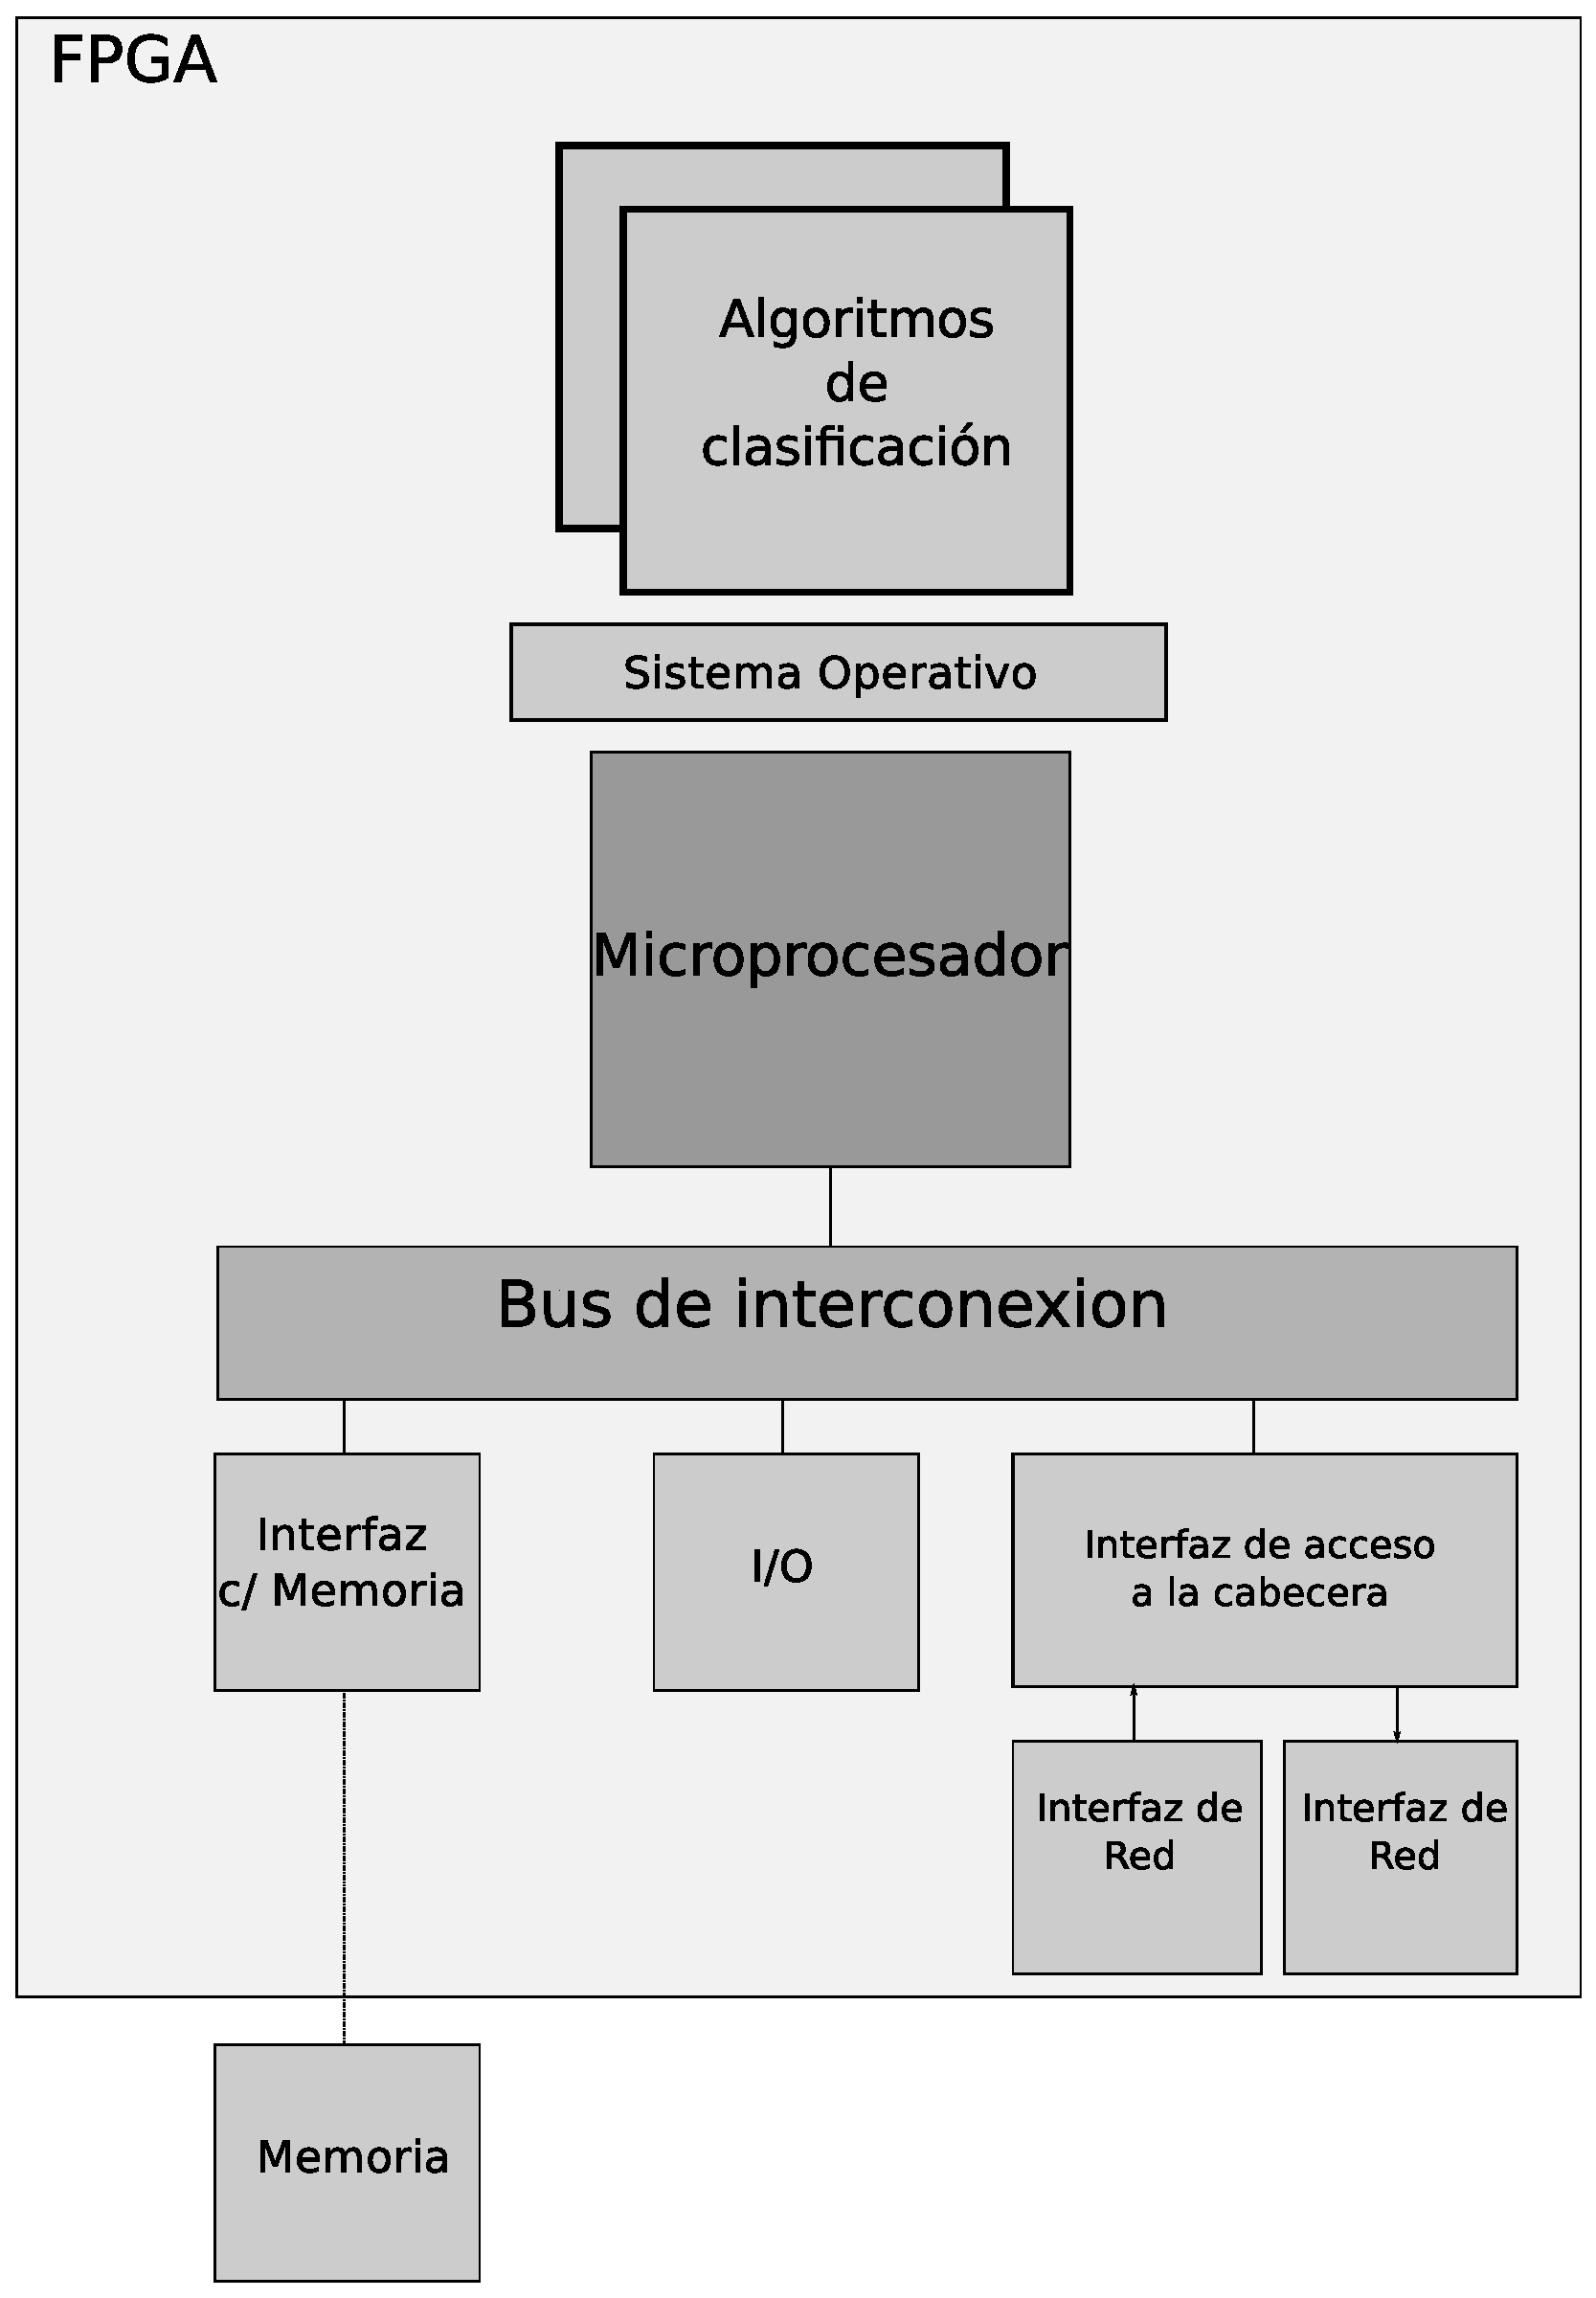
\includegraphics[width=0.6\textwidth]{2-sistema/graf/solucion.eps}
  \caption{Diagrama de la arquitectura propuesta}
  \label{fig:solucion}
\end{figure}

De los módulos mencionados, es necesario poner especial atención en el diseño de la interfaz de acceso a la cabecera.

\subsection{Interfaz de acceso a la cabecera}
Este módulo tiene como función acceder a los campos que conforman la cabecera IP en los paquetes entrantes. La información recolectada es enviada al microprocesador para que este implemente el software de clasificación.

\newpage

 \begin{figure}[h]
  \centering
	 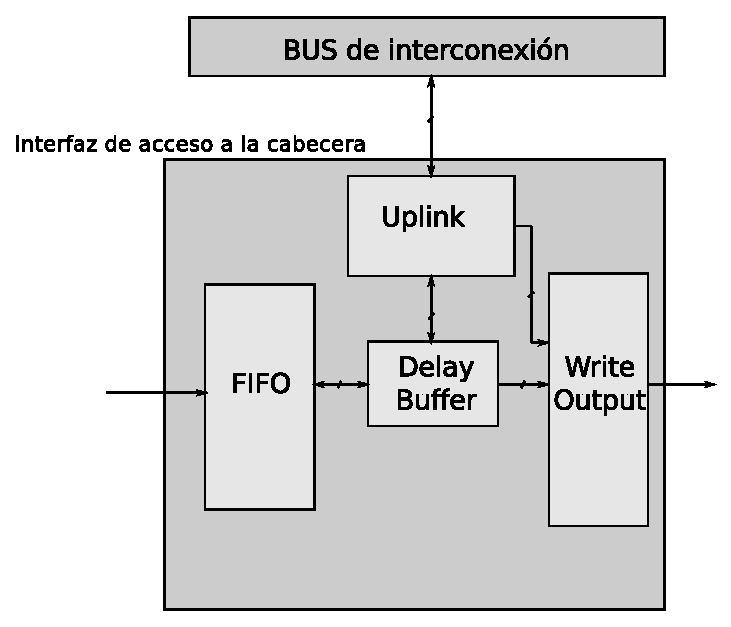
\includegraphics[width=0.6\textwidth]{2-sistema/graf/modulo.eps}
  \caption{Interfaz de acceso a la cabecera}
  \label{fig:inter}
\end{figure}



%\subsection{Descripción funcional}

A continuación se describe funcionalmente cada uno de los bloques que conforma la interfaz, ilustrada en la figura~\ref{fig:inter}
\subsubsection{Cola de espera FIFO\textit{(First in First out)}}
A la entrada del módulo se encuentra una FIFO que se encarga de almacenar y poner a disposición en orden de llegada los datos que emite el generador. Además, para poder manipular los paquetes, la FIFO debe almacenar toda la información de control disponible a su entrada.
Este módulo también debe permitir la parametrización en la mayor cantidad de sentidos posibles, especialmente se desea poder configurar la cantidad de palabras a almacenar, ya que la memoria dentro de un FPGA es un recurso crítico y se desea encontrar la mejor relación entre rendimiento y consumo de recursos.

\subsubsection{Delay Buffer}
Este componente será el encargado de ir tomando los datos desde la FIFO y de detectar el inicio y finalización de un paquete. Además deberá mantener almacenada la cabecera del paquete mientras el software toma una decisión. En este módulo es deseable configurar la cantidad de palabras que se considerarán parte de la cabecera y que serán enviadas al microprocesador.

\subsubsection{Uplink}
Este módulo es el encargado de gestionar las transacciones con el microprocesador. Para ello debe entender las señales que utiliza el bus y poder interrumpir al procesador para enviarle los datos cuando estos estén disponibles. Asimismo cuando el procesador responde con el resultado de la clasificación, Uplink lo almacena y lo envía al módulo Write output para que este escriba el resultado de la clasificación en la etiqueta anexa al paquete correspondiente.
Eventualmente se desarrollaran varias versiones de este módulo, que envíen toda la cabecera o una parte selectiva de ella buscando optimizar el rendimiento.

\subsubsection{Write Output}
Para finalizar este módulo toma la salida de Delay Buffer y escribe el resultado que le envía Uplink en la etiqueta que se encuentra anexa a cada una de las palabras del paquete.

\section{Algoritmos de Clasificación}

Los algoritmos de clasificación de paquetes que se implementaron fueron los siguientes:

\subsection{Búsqueda lineal}

El esquema más simple de lookup consiste en una tabla, donde cada entrada contiene un prefijo (expresado en notación máscara) mas un identificador de enlace de salida. Cuando llega un paquete se examina su dirección IP y se va comparando con cada uno de los prefijos almacenados. Para que exista correspondencia debe existir igualdad bit a bit entre el prefijo y la dirección IP. Si esto se cumple para varios prefijos, se opta por el más largo de ellos y el paquete se expide por el enlace asociado a dicho prefijo.
Para optimizar este esquema, los prefijos se almacenan en orden decreciente de longitud, como se muestra en la figura~\ref{fig:linear}, de manera que al encontrar una coincidencia no sea necesario seguir buscando en el resto de la tabla. 

\begin{figure}[h]
  \centering
	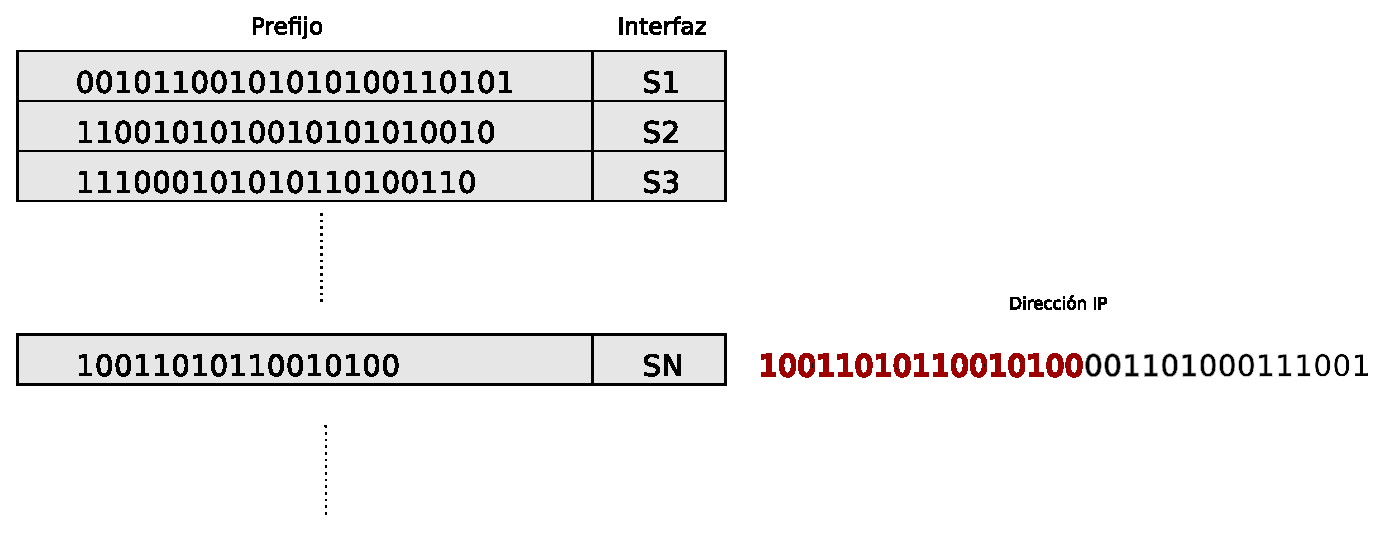
\includegraphics[width=0.80\textwidth]{2-sistema/graf/linear.eps}
  \caption{Búsqueda lineal}
  \label{fig:linear}
\end{figure}

\newpage
\subsection {Unibit tries}

Un Unibit trie es un árbol en el cual cada nodo contiene un \textit{puntero-cero }y un \textit{puntero-uno}. Partiendo del nodo raíz, todos los prefijos que comienzan con 0 son almacenados en el subárbol apuntado por el puntero-cero y aquellos que comienzan con 1 se almacenan en el subárbol apuntado por el puntero-uno.Cada subárbol es construido recursivamente de manera similar usando los bits restantes de cada uno de los prefijos.
Considerar la siguiente tabla de enrutamiento:
\begin{table}[h]
\begin{center}
	\begin{tabular}{|c|c|} \hline
		\textbf{Prefijo} & \textbf{Enlace de salida} \\ \hline
		101* & S1 \\
		111* & S2 \\
		11001* & S3 \\
		1* & S4 \\
		0* & S5 \\
		1000* & S6 \\
		100000* & S7 \\
		100* & S8 \\
		110* & S9 \\	\hline
	\end{tabular}
	\caption{Prefijos y enlaces de salida}
	\label{tab:prefgw}	
\end{center}
\end{table}



A la misma le corresponde la representación en Unibit trie de la figura~\ref{fig:trie}.
Sea una dirección de destino \textit{D}. Para efectuar la búsqueda del prefijo más largo, los bits de \textit{D} son usados para trazar un camino a lo largo del trie. Dicho camino comienza en el nodo raíz y continúa hasta encontrar un puntero vacío o un nodo vacío. Durante el recorrido a través del trie, el algoritmo mantiene un registro del último enlace encontrado en un nodo del camino recorrido (que es el mas largo hasta el momento). En el caso que la búsqueda terminara éste es el prefijo retornado.

\begin{figure}[h]
  \centering
	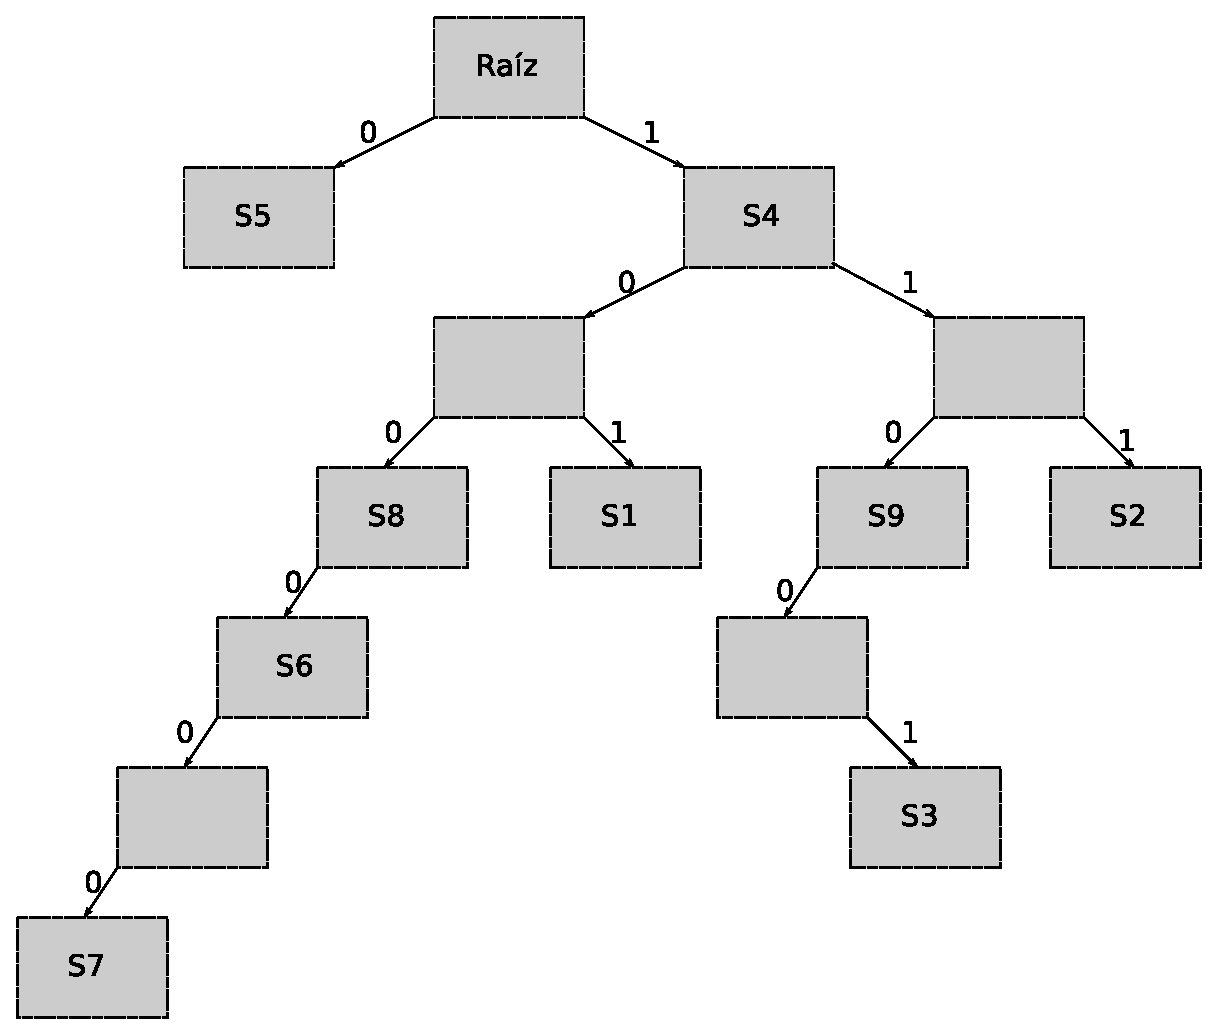
\includegraphics[width=0.80\textwidth]{2-sistema/graf/trie.eps}
  \caption{Unibit trie}
  \label{fig:trie}
\end{figure}


